Dagli spazi vettoriali dall'algebra lineare agli spazi vettoriali in cui le basi sono funzioni (spazi di Hilbert).
Per fare questo passaggio ripassiamo i vettori.

\section{Rappresentazione}
Esistono due tipi di rappresentazione, cartesiana e polare.

\begin{figure}[ht!]
    \centering
    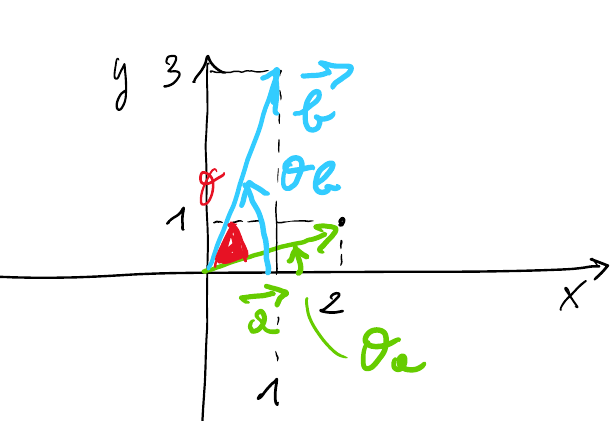
\includegraphics[scale=0.35]{immagini/lez7/vettori.jpg}
\end{figure}

\[\begin{split}
    \Vec{a} =
    \begin{pmatrix}
    2\\
    1
    \end{pmatrix}
    \mbox{  }|\Vec{a}| &= \sqrt{1+4} = \sqrt{5} \\
    \Theta_a &= arctan \frac{1}{2} \\
    \Vec{b} =
    \begin{pmatrix}
    1\\
    3
    \end{pmatrix}
    \mbox{  }|\Vec{b}| &= \sqrt{1+9} = \sqrt{10} \\
    \Theta_b &= arctan 3
\end{split}
\]

\section{Prodotto Scalare}
Il prodotto scalare di due vettori e' la loro combinazione lineare (il primo elemento del primo vettore moltiplicato per il primo elemento del secondo vettore, e cosi' via). Il risultato e' un numero ed il simbolo e' $\langle\Vec{a}, \Vec{b}\rangle$ o $\Vec{a} \cdot \Vec{b}$.

\begin{figure}[ht!]
    \centering
    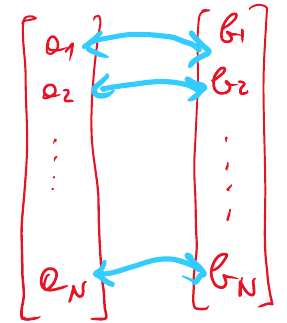
\includegraphics[scale=0.35]{immagini/lez7/prodottoScalare.jpg}
\end{figure}

Rappresentazione cartesiana:
\[\begin{split}
    [2, 1] [1, 3] = 2 \cdot 1 + 1 \cdot 3 = 5
\end{split}\]

\section{Vettori ortogonali}
Due vettori sono ortogonali quando il loro prodotto scalare e' zero.

\begin{figure}[ht!]
    \centering
    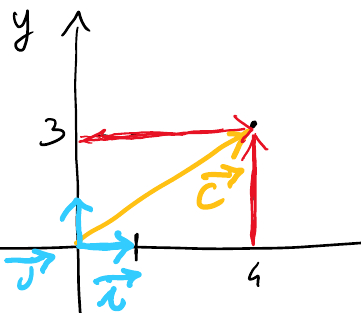
\includegraphics[scale=0.35]{immagini/lez7/vettoriOrtogonali.jpg}
\end{figure}

i e j sono detti VERSORI, posso riscrivere il vettore C come combinazione dei versori:

\[
    \Vec{C} = \Vec{i} 4 + \Vec{j} \cdot 3 
\]

Di conseguenza possiamo considerare C come combinazione lineare delle basi nello spazio vettoriale e il modulo del vettore e' la sua proiezione ortogonale.
Quindi riconducendo questo discorso ai segnali, ogni volta che analizziamo un vettore ne facciamo il prodotto scalare dal prodotto scalare per fare una "sintesi" del vettore rimetto insieme i prodotti scalari.